% Options for packages loaded elsewhere
\PassOptionsToPackage{unicode}{hyperref}
\PassOptionsToPackage{hyphens}{url}
\PassOptionsToPackage{dvipsnames,svgnames,x11names}{xcolor}
%
\documentclass[
  letterpaper,
  DIV=11,
  numbers=noendperiod]{scrartcl}

\usepackage{amsmath,amssymb}
\usepackage{iftex}
\ifPDFTeX
  \usepackage[T1]{fontenc}
  \usepackage[utf8]{inputenc}
  \usepackage{textcomp} % provide euro and other symbols
\else % if luatex or xetex
  \usepackage{unicode-math}
  \defaultfontfeatures{Scale=MatchLowercase}
  \defaultfontfeatures[\rmfamily]{Ligatures=TeX,Scale=1}
\fi
\usepackage{lmodern}
\ifPDFTeX\else  
    % xetex/luatex font selection
\fi
% Use upquote if available, for straight quotes in verbatim environments
\IfFileExists{upquote.sty}{\usepackage{upquote}}{}
\IfFileExists{microtype.sty}{% use microtype if available
  \usepackage[]{microtype}
  \UseMicrotypeSet[protrusion]{basicmath} % disable protrusion for tt fonts
}{}
\makeatletter
\@ifundefined{KOMAClassName}{% if non-KOMA class
  \IfFileExists{parskip.sty}{%
    \usepackage{parskip}
  }{% else
    \setlength{\parindent}{0pt}
    \setlength{\parskip}{6pt plus 2pt minus 1pt}}
}{% if KOMA class
  \KOMAoptions{parskip=half}}
\makeatother
\usepackage{xcolor}
\setlength{\emergencystretch}{3em} % prevent overfull lines
\setcounter{secnumdepth}{-\maxdimen} % remove section numbering
% Make \paragraph and \subparagraph free-standing
\makeatletter
\ifx\paragraph\undefined\else
  \let\oldparagraph\paragraph
  \renewcommand{\paragraph}{
    \@ifstar
      \xxxParagraphStar
      \xxxParagraphNoStar
  }
  \newcommand{\xxxParagraphStar}[1]{\oldparagraph*{#1}\mbox{}}
  \newcommand{\xxxParagraphNoStar}[1]{\oldparagraph{#1}\mbox{}}
\fi
\ifx\subparagraph\undefined\else
  \let\oldsubparagraph\subparagraph
  \renewcommand{\subparagraph}{
    \@ifstar
      \xxxSubParagraphStar
      \xxxSubParagraphNoStar
  }
  \newcommand{\xxxSubParagraphStar}[1]{\oldsubparagraph*{#1}\mbox{}}
  \newcommand{\xxxSubParagraphNoStar}[1]{\oldsubparagraph{#1}\mbox{}}
\fi
\makeatother

\usepackage{color}
\usepackage{fancyvrb}
\newcommand{\VerbBar}{|}
\newcommand{\VERB}{\Verb[commandchars=\\\{\}]}
\DefineVerbatimEnvironment{Highlighting}{Verbatim}{commandchars=\\\{\}}
% Add ',fontsize=\small' for more characters per line
\usepackage{framed}
\definecolor{shadecolor}{RGB}{241,243,245}
\newenvironment{Shaded}{\begin{snugshade}}{\end{snugshade}}
\newcommand{\AlertTok}[1]{\textcolor[rgb]{0.68,0.00,0.00}{#1}}
\newcommand{\AnnotationTok}[1]{\textcolor[rgb]{0.37,0.37,0.37}{#1}}
\newcommand{\AttributeTok}[1]{\textcolor[rgb]{0.40,0.45,0.13}{#1}}
\newcommand{\BaseNTok}[1]{\textcolor[rgb]{0.68,0.00,0.00}{#1}}
\newcommand{\BuiltInTok}[1]{\textcolor[rgb]{0.00,0.23,0.31}{#1}}
\newcommand{\CharTok}[1]{\textcolor[rgb]{0.13,0.47,0.30}{#1}}
\newcommand{\CommentTok}[1]{\textcolor[rgb]{0.37,0.37,0.37}{#1}}
\newcommand{\CommentVarTok}[1]{\textcolor[rgb]{0.37,0.37,0.37}{\textit{#1}}}
\newcommand{\ConstantTok}[1]{\textcolor[rgb]{0.56,0.35,0.01}{#1}}
\newcommand{\ControlFlowTok}[1]{\textcolor[rgb]{0.00,0.23,0.31}{\textbf{#1}}}
\newcommand{\DataTypeTok}[1]{\textcolor[rgb]{0.68,0.00,0.00}{#1}}
\newcommand{\DecValTok}[1]{\textcolor[rgb]{0.68,0.00,0.00}{#1}}
\newcommand{\DocumentationTok}[1]{\textcolor[rgb]{0.37,0.37,0.37}{\textit{#1}}}
\newcommand{\ErrorTok}[1]{\textcolor[rgb]{0.68,0.00,0.00}{#1}}
\newcommand{\ExtensionTok}[1]{\textcolor[rgb]{0.00,0.23,0.31}{#1}}
\newcommand{\FloatTok}[1]{\textcolor[rgb]{0.68,0.00,0.00}{#1}}
\newcommand{\FunctionTok}[1]{\textcolor[rgb]{0.28,0.35,0.67}{#1}}
\newcommand{\ImportTok}[1]{\textcolor[rgb]{0.00,0.46,0.62}{#1}}
\newcommand{\InformationTok}[1]{\textcolor[rgb]{0.37,0.37,0.37}{#1}}
\newcommand{\KeywordTok}[1]{\textcolor[rgb]{0.00,0.23,0.31}{\textbf{#1}}}
\newcommand{\NormalTok}[1]{\textcolor[rgb]{0.00,0.23,0.31}{#1}}
\newcommand{\OperatorTok}[1]{\textcolor[rgb]{0.37,0.37,0.37}{#1}}
\newcommand{\OtherTok}[1]{\textcolor[rgb]{0.00,0.23,0.31}{#1}}
\newcommand{\PreprocessorTok}[1]{\textcolor[rgb]{0.68,0.00,0.00}{#1}}
\newcommand{\RegionMarkerTok}[1]{\textcolor[rgb]{0.00,0.23,0.31}{#1}}
\newcommand{\SpecialCharTok}[1]{\textcolor[rgb]{0.37,0.37,0.37}{#1}}
\newcommand{\SpecialStringTok}[1]{\textcolor[rgb]{0.13,0.47,0.30}{#1}}
\newcommand{\StringTok}[1]{\textcolor[rgb]{0.13,0.47,0.30}{#1}}
\newcommand{\VariableTok}[1]{\textcolor[rgb]{0.07,0.07,0.07}{#1}}
\newcommand{\VerbatimStringTok}[1]{\textcolor[rgb]{0.13,0.47,0.30}{#1}}
\newcommand{\WarningTok}[1]{\textcolor[rgb]{0.37,0.37,0.37}{\textit{#1}}}

\providecommand{\tightlist}{%
  \setlength{\itemsep}{0pt}\setlength{\parskip}{0pt}}\usepackage{longtable,booktabs,array}
\usepackage{calc} % for calculating minipage widths
% Correct order of tables after \paragraph or \subparagraph
\usepackage{etoolbox}
\makeatletter
\patchcmd\longtable{\par}{\if@noskipsec\mbox{}\fi\par}{}{}
\makeatother
% Allow footnotes in longtable head/foot
\IfFileExists{footnotehyper.sty}{\usepackage{footnotehyper}}{\usepackage{footnote}}
\makesavenoteenv{longtable}
\usepackage{graphicx}
\makeatletter
\newsavebox\pandoc@box
\newcommand*\pandocbounded[1]{% scales image to fit in text height/width
  \sbox\pandoc@box{#1}%
  \Gscale@div\@tempa{\textheight}{\dimexpr\ht\pandoc@box+\dp\pandoc@box\relax}%
  \Gscale@div\@tempb{\linewidth}{\wd\pandoc@box}%
  \ifdim\@tempb\p@<\@tempa\p@\let\@tempa\@tempb\fi% select the smaller of both
  \ifdim\@tempa\p@<\p@\scalebox{\@tempa}{\usebox\pandoc@box}%
  \else\usebox{\pandoc@box}%
  \fi%
}
% Set default figure placement to htbp
\def\fps@figure{htbp}
\makeatother

\usepackage{booktabs}
\usepackage{caption}
\usepackage{longtable}
\usepackage{colortbl}
\usepackage{array}
\usepackage{anyfontsize}
\usepackage{multirow}
\KOMAoption{captions}{tableheading}
\makeatletter
\@ifpackageloaded{caption}{}{\usepackage{caption}}
\AtBeginDocument{%
\ifdefined\contentsname
  \renewcommand*\contentsname{Table of contents}
\else
  \newcommand\contentsname{Table of contents}
\fi
\ifdefined\listfigurename
  \renewcommand*\listfigurename{List of Figures}
\else
  \newcommand\listfigurename{List of Figures}
\fi
\ifdefined\listtablename
  \renewcommand*\listtablename{List of Tables}
\else
  \newcommand\listtablename{List of Tables}
\fi
\ifdefined\figurename
  \renewcommand*\figurename{Figure}
\else
  \newcommand\figurename{Figure}
\fi
\ifdefined\tablename
  \renewcommand*\tablename{Table}
\else
  \newcommand\tablename{Table}
\fi
}
\@ifpackageloaded{float}{}{\usepackage{float}}
\floatstyle{ruled}
\@ifundefined{c@chapter}{\newfloat{codelisting}{h}{lop}}{\newfloat{codelisting}{h}{lop}[chapter]}
\floatname{codelisting}{Listing}
\newcommand*\listoflistings{\listof{codelisting}{List of Listings}}
\makeatother
\makeatletter
\makeatother
\makeatletter
\@ifpackageloaded{caption}{}{\usepackage{caption}}
\@ifpackageloaded{subcaption}{}{\usepackage{subcaption}}
\makeatother

\usepackage{bookmark}

\IfFileExists{xurl.sty}{\usepackage{xurl}}{} % add URL line breaks if available
\urlstyle{same} % disable monospaced font for URLs
\hypersetup{
  pdftitle={Final EDA},
  pdfauthor={Julia Vitale, Mia Zottoli, and Vishnu Lakshman},
  colorlinks=true,
  linkcolor={blue},
  filecolor={Maroon},
  citecolor={Blue},
  urlcolor={Blue},
  pdfcreator={LaTeX via pandoc}}


\title{Final EDA}
\author{Julia Vitale, Mia Zottoli, and Vishnu Lakshman}
\date{}

\begin{document}
\maketitle


\begin{Shaded}
\begin{Highlighting}[]
\FunctionTok{library}\NormalTok{(here)}
\end{Highlighting}
\end{Shaded}

\begin{verbatim}
Warning: package 'here' was built under R version 4.4.2
\end{verbatim}

\begin{verbatim}
here() starts at C:/Users/anne/Documents/m255/M244-Final-JVM
\end{verbatim}

\begin{Shaded}
\begin{Highlighting}[]
\FunctionTok{library}\NormalTok{(tidyverse)}
\end{Highlighting}
\end{Shaded}

\begin{verbatim}
Warning: package 'tidyverse' was built under R version 4.4.2
\end{verbatim}

\begin{verbatim}
Warning: package 'ggplot2' was built under R version 4.4.2
\end{verbatim}

\begin{verbatim}
Warning: package 'tibble' was built under R version 4.4.2
\end{verbatim}

\begin{verbatim}
Warning: package 'tidyr' was built under R version 4.4.2
\end{verbatim}

\begin{verbatim}
Warning: package 'readr' was built under R version 4.4.2
\end{verbatim}

\begin{verbatim}
Warning: package 'purrr' was built under R version 4.4.2
\end{verbatim}

\begin{verbatim}
Warning: package 'dplyr' was built under R version 4.4.2
\end{verbatim}

\begin{verbatim}
Warning: package 'stringr' was built under R version 4.4.2
\end{verbatim}

\begin{verbatim}
Warning: package 'forcats' was built under R version 4.4.2
\end{verbatim}

\begin{verbatim}
Warning: package 'lubridate' was built under R version 4.4.2
\end{verbatim}

\begin{verbatim}
-- Attaching core tidyverse packages ------------------------ tidyverse 2.0.0 --
v dplyr     1.1.4     v readr     2.1.5
v forcats   1.0.0     v stringr   1.5.1
v ggplot2   3.5.1     v tibble    3.2.1
v lubridate 1.9.4     v tidyr     1.3.1
v purrr     1.0.2     
\end{verbatim}

\begin{verbatim}
-- Conflicts ------------------------------------------ tidyverse_conflicts() --
x dplyr::filter() masks stats::filter()
x dplyr::lag()    masks stats::lag()
i Use the conflicted package (<http://conflicted.r-lib.org/>) to force all conflicts to become errors
\end{verbatim}

\begin{Shaded}
\begin{Highlighting}[]
\FunctionTok{library}\NormalTok{(ggplot2)}
\end{Highlighting}
\end{Shaded}

\begin{Shaded}
\begin{Highlighting}[]
\NormalTok{ultimate\_data }\OtherTok{\textless{}{-}} \FunctionTok{read\_csv}\NormalTok{(}\FunctionTok{here}\NormalTok{(}\StringTok{"data"}\NormalTok{, }\StringTok{"ultimate\_college\_championship.csv"}\NormalTok{)) }\SpecialCharTok{\%\textgreater{}\%}
  \FunctionTok{mutate}\NormalTok{(}\FunctionTok{across}\NormalTok{(}\FunctionTok{c}\NormalTok{(level, gender, division, team\_name), as.factor)) }\SpecialCharTok{\%\textgreater{}\%}
  \FunctionTok{mutate}\NormalTok{(}\AttributeTok{school =} \FunctionTok{str\_split\_i}\NormalTok{(team\_name, }\StringTok{" "}\NormalTok{, }\DecValTok{1}\NormalTok{)) }\SpecialCharTok{\%\textgreater{}\%}
  \FunctionTok{mutate}\NormalTok{(}\AttributeTok{school =} \FunctionTok{ifelse}\NormalTok{(}\FunctionTok{str\_detect}\NormalTok{(team\_name, }\StringTok{"St Olaf"}\NormalTok{), }\StringTok{"St Olaf"}\NormalTok{, school)) }\SpecialCharTok{\%\textgreater{}\%}
  \FunctionTok{mutate}\NormalTok{(}\AttributeTok{school =} \FunctionTok{ifelse}\NormalTok{(}\FunctionTok{str\_detect}\NormalTok{(team\_name, }\StringTok{"North Carolina"}\NormalTok{), }\StringTok{"North Carolina"}\NormalTok{, school)) }\SpecialCharTok{\%\textgreater{}\%}
  \FunctionTok{mutate}\NormalTok{(}\AttributeTok{school =} \FunctionTok{ifelse}\NormalTok{(}\FunctionTok{str\_detect}\NormalTok{(team\_name, }\StringTok{"Cal Poly"}\NormalTok{), }\StringTok{"Cal Poly SLO"}\NormalTok{, school))  }\SpecialCharTok{\%\textgreater{}\%}
  \FunctionTok{mutate}\NormalTok{(}\AttributeTok{school =} \FunctionTok{ifelse}\NormalTok{(}\FunctionTok{str\_detect}\NormalTok{(team\_name, }\StringTok{"British Columbia"}\NormalTok{), }\StringTok{"British Columbia"}\NormalTok{, school))  }\SpecialCharTok{\%\textgreater{}\%}
  \FunctionTok{mutate}\NormalTok{(}\AttributeTok{school =} \FunctionTok{ifelse}\NormalTok{(}\FunctionTok{str\_detect}\NormalTok{(team\_name, }\StringTok{"Western Washington"}\NormalTok{), }\StringTok{"Western Washington"}\NormalTok{, school))  }\SpecialCharTok{\%\textgreater{}\%}
  \FunctionTok{mutate}\NormalTok{(}\AttributeTok{school =} \FunctionTok{ifelse}\NormalTok{(}\FunctionTok{str\_detect}\NormalTok{(team\_name, }\StringTok{"Penn State"}\NormalTok{), }\StringTok{"Penn State"}\NormalTok{, school))  }\SpecialCharTok{\%\textgreater{}\%}
  \FunctionTok{mutate}\NormalTok{(}\AttributeTok{school =} \FunctionTok{ifelse}\NormalTok{(}\FunctionTok{str\_detect}\NormalTok{(team\_name, }\StringTok{"San Diego"}\NormalTok{), }\StringTok{"UCSD"}\NormalTok{, school))  }\SpecialCharTok{\%\textgreater{}\%}
  \FunctionTok{mutate}\NormalTok{(}\AttributeTok{school =} \FunctionTok{ifelse}\NormalTok{(}\FunctionTok{str\_detect}\NormalTok{(team\_name, }\StringTok{"Lewis"}\NormalTok{), }\StringTok{"Lewis \& Clark"}\NormalTok{, school))  }\SpecialCharTok{\%\textgreater{}\%}
  \FunctionTok{mutate}\NormalTok{(}\AttributeTok{school =} \FunctionTok{ifelse}\NormalTok{(}\FunctionTok{str\_detect}\NormalTok{(team\_name, }\StringTok{"Colorado State"}\NormalTok{), }\StringTok{"Colorado State"}\NormalTok{, school))  }\SpecialCharTok{\%\textgreater{}\%}
  \FunctionTok{mutate}\NormalTok{(}\AttributeTok{school =} \FunctionTok{ifelse}\NormalTok{(}\FunctionTok{str\_detect}\NormalTok{(team\_name, }\StringTok{"Oklahoma Christian"}\NormalTok{), }\StringTok{"Oklahoma Christian"}\NormalTok{, school))  }\SpecialCharTok{\%\textgreater{}\%}
  \FunctionTok{mutate}\NormalTok{(}\AttributeTok{school =} \FunctionTok{ifelse}\NormalTok{(}\FunctionTok{str\_detect}\NormalTok{(team\_name, }\StringTok{"Binghamton"}\NormalTok{), }\StringTok{"SUNY Binghamton"}\NormalTok{, school))  }\SpecialCharTok{\%\textgreater{}\%}
  \FunctionTok{mutate}\NormalTok{(}\AttributeTok{school =} \FunctionTok{ifelse}\NormalTok{(}\FunctionTok{str\_detect}\NormalTok{(team\_name, }\StringTok{"Santa Bar"}\NormalTok{), }\StringTok{"UCSB"}\NormalTok{, school))  }\SpecialCharTok{\%\textgreater{}\%}
  \FunctionTok{mutate}\NormalTok{(}\AttributeTok{school =} \FunctionTok{ifelse}\NormalTok{(}\FunctionTok{str\_detect}\NormalTok{(team\_name, }\StringTok{"Santa Cr"}\NormalTok{), }\StringTok{"USCS"}\NormalTok{, school))  }\SpecialCharTok{\%\textgreater{}\%}
  \FunctionTok{mutate}\NormalTok{(}\AttributeTok{school =} \FunctionTok{ifelse}\NormalTok{(}\FunctionTok{str\_detect}\NormalTok{(team\_name, }\StringTok{"Colorado College"}\NormalTok{), }\StringTok{"Colorado College"}\NormalTok{, school))  }\SpecialCharTok{\%\textgreater{}\%}
  \FunctionTok{mutate}\NormalTok{(}\AttributeTok{school =} \FunctionTok{ifelse}\NormalTok{(}\FunctionTok{str\_detect}\NormalTok{(team\_name, }\StringTok{"Missouri S"}\NormalTok{), }\StringTok{"Missouri S\&T"}\NormalTok{, school))  }\SpecialCharTok{\%\textgreater{}\%}
  \FunctionTok{mutate}\NormalTok{(}\AttributeTok{school =} \FunctionTok{ifelse}\NormalTok{(}\FunctionTok{str\_detect}\NormalTok{(team\_name, }\StringTok{"Holyoke"}\NormalTok{), }\StringTok{"Mount Holyoke"}\NormalTok{, school))  }\SpecialCharTok{\%\textgreater{}\%}
  \FunctionTok{mutate}\NormalTok{(}\AttributeTok{school =} \FunctionTok{ifelse}\NormalTok{(}\FunctionTok{str\_detect}\NormalTok{(team\_name, }\StringTok{"NC State"}\NormalTok{), }\StringTok{"NC State"}\NormalTok{, school))  }\SpecialCharTok{\%\textgreater{}\%}
  \FunctionTok{mutate}\NormalTok{(}\AttributeTok{school =} \FunctionTok{ifelse}\NormalTok{(}\FunctionTok{str\_detect}\NormalTok{(team\_name, }\StringTok{"Oregon State"}\NormalTok{), }\StringTok{"Oregon State"}\NormalTok{, school))  }\SpecialCharTok{\%\textgreater{}\%}
  \FunctionTok{mutate}\NormalTok{(}\AttributeTok{school =} \FunctionTok{ifelse}\NormalTok{(}\FunctionTok{str\_detect}\NormalTok{(team\_name, }\StringTok{"Washington University"}\NormalTok{), }\StringTok{"Washington University"}\NormalTok{, school))}
\end{Highlighting}
\end{Shaded}

\begin{verbatim}
Rows: 1665 Columns: 16
-- Column specification --------------------------------------------------------
Delimiter: ","
chr  (5): player, level, gender, division, team_name
dbl (11): Turns, Ds, Assists, Points, plus_minus, team_games, turns_per_game...

i Use `spec()` to retrieve the full column specification for this data.
i Specify the column types or set `show_col_types = FALSE` to quiet this message.
\end{verbatim}

\subsection{Exploring the Data}\label{exploring-the-data}

Answer the following questions:

\begin{itemize}
\tightlist
\item
  What is your outcome variable(s)? How well does it measure the outcome
  you are interested? How does it relate to your expectations?
\end{itemize}

\emph{Our outcome variable is plus\_minus, which is the difference
between the amount of points scored by an individual player's team while
that player is on the field and the amount of points scored by the
opposing team while that player is on the field. We are interested in
the influence of an individual player on the success of the whole team,
so this variable is a good measure of our outcome of interest.}

\emph{Essentially, +/- for a select player = points scored by player's
team (while player is on the field) - points scored by opposing team
(while player is on the field)}

\emph{The +/- score is used to track a player's overall effectiveness on
the field and their impact on the game. A positive +/- score means the
player's team scored more than the opposing team while the player was on
the field, and a negative +/- score means the opposing team scored more
while the player was on the field.}

\begin{itemize}
\item
  What are your key explanatory variables?

  \emph{Turns (turnovers) per game, points scored per game, Ds
  (defensive interceptions) per game, level (Division 1 or 3), division
  (Men's or Women's) and school.}
\end{itemize}

In addition, create a table of summary statistics for the variables you
are planning to use.

\begin{Shaded}
\begin{Highlighting}[]
\NormalTok{ultimate\_data }\SpecialCharTok{\%\textgreater{}\%} \FunctionTok{select}\NormalTok{(}\SpecialCharTok{{-}}\FunctionTok{c}\NormalTok{(player, team\_name)) }\SpecialCharTok{\%\textgreater{}\%}\NormalTok{ gtsummary}\SpecialCharTok{::}\FunctionTok{tbl\_summary}\NormalTok{()}
\end{Highlighting}
\end{Shaded}

\begin{table}
\fontsize{12.0pt}{14.4pt}\selectfont
\begin{tabular*}{\linewidth}{@{\extracolsep{\fill}}lc}
\toprule
\textbf{Characteristic} & \textbf{N = 1,665}\textsuperscript{\textit{1}} \\ 
\midrule\addlinespace[2.5pt]
level &  \\ 
    Division 1 & 973 (58\%) \\ 
    Division 3 & 692 (42\%) \\ 
gender &  \\ 
    Men & 893 (54\%) \\ 
    Women & 772 (46\%) \\ 
division &  \\ 
    Division 1 Men & 521 (31\%) \\ 
    Division 1 Women & 452 (27\%) \\ 
    Division 3 Men & 372 (22\%) \\ 
    Division 3 Women & 320 (19\%) \\ 
Turns & 2 (0, 7) \\ 
Ds & 1.00 (0.00, 3.00) \\ 
Assists & 1.0 (0.0, 3.0) \\ 
Points & 1.0 (0.0, 4.0) \\ 
plus\_minus & 1 (0, 5) \\ 
team\_games &  \\ 
    5 & 780 (47\%) \\ 
    6 & 738 (44\%) \\ 
    7 & 122 (7.3\%) \\ 
    8 & 25 (1.5\%) \\ 
turns\_per\_game & 0.40 (0.00, 1.17) \\ 
ds\_per\_game & 0.20 (0.00, 0.50) \\ 
ast\_per\_game & 0.17 (0.00, 0.60) \\ 
pts\_per\_game & 0.20 (0.00, 0.71) \\ 
pls\_mns\_per\_game & 0.20 (0.00, 0.83) \\ 
school &  \\ 
    Alabama-Huntsville & 23 (1.4\%) \\ 
    Bates & 17 (1.0\%) \\ 
    Berry & 26 (1.6\%) \\ 
    British Columbia & 23 (1.4\%) \\ 
    Brown & 25 (1.5\%) \\ 
    Cal & 23 (1.4\%) \\ 
    Cal Poly SLO & 24 (1.4\%) \\ 
    Carleton & 101 (6.1\%) \\ 
    Claremont & 24 (1.4\%) \\ 
    Colorado & 49 (2.9\%) \\ 
    Colorado College & 22 (1.3\%) \\ 
    Colorado State & 21 (1.3\%) \\ 
    Davenport & 31 (1.9\%) \\ 
    Franciscan & 22 (1.3\%) \\ 
    Georgia & 45 (2.7\%) \\ 
    Grinnell & 15 (0.9\%) \\ 
    Haverford/Bryn & 24 (1.4\%) \\ 
    Lewis \& Clark & 44 (2.6\%) \\ 
    Macalester & 20 (1.2\%) \\ 
    Massachusetts & 28 (1.7\%) \\ 
    Michigan & 54 (3.2\%) \\ 
    Middlebury & 53 (3.2\%) \\ 
    Minnesota & 28 (1.7\%) \\ 
    Missouri S\&T & 15 (0.9\%) \\ 
    Mount Holyoke & 12 (0.7\%) \\ 
    NC State & 30 (1.8\%) \\ 
    North Carolina & 61 (3.7\%) \\ 
    Oberlin & 22 (1.3\%) \\ 
    Occidental & 23 (1.4\%) \\ 
    Oklahoma Christian & 24 (1.4\%) \\ 
    Oregon & 51 (3.1\%) \\ 
    Oregon State & 22 (1.3\%) \\ 
    Ottawa & 16 (1.0\%) \\ 
    Penn State & 24 (1.4\%) \\ 
    Pennsylvania & 22 (1.3\%) \\ 
    Pittsburgh & 28 (1.7\%) \\ 
    Portland & 24 (1.4\%) \\ 
    Richmond & 39 (2.3\%) \\ 
    Rochester & 25 (1.5\%) \\ 
    St Olaf & 51 (3.1\%) \\ 
    Stanford & 22 (1.3\%) \\ 
    SUNY Binghamton & 22 (1.3\%) \\ 
    Texas & 26 (1.6\%) \\ 
    Tufts & 21 (1.3\%) \\ 
    UCSB & 23 (1.4\%) \\ 
    UCSD & 25 (1.5\%) \\ 
    Union & 18 (1.1\%) \\ 
    USCS & 21 (1.3\%) \\ 
    Utah & 22 (1.3\%) \\ 
    Vermont & 46 (2.8\%) \\ 
    Victoria & 20 (1.2\%) \\ 
    Washington & 26 (1.6\%) \\ 
    Washington University & 29 (1.7\%) \\ 
    Wellesley & 20 (1.2\%) \\ 
    Wesleyan & 22 (1.3\%) \\ 
    Western Washington & 23 (1.4\%) \\ 
    Whitman & 22 (1.3\%) \\ 
    Williams & 26 (1.6\%) \\ 
\bottomrule
\end{tabular*}
\begin{minipage}{\linewidth}
\textsuperscript{\textit{1}}n (\%); Median (Q1, Q3)\\
\end{minipage}
\end{table}

\subsection{Data Wrangling and
Transformation}\label{data-wrangling-and-transformation}

Answer the following question:

\begin{itemize}
\tightlist
\item
  What data cleaning did you have to do?
\item
  How did you wrangle the data?
\item
  Are you deciding to exclude any observations? If so, why?
\item
  Did you have to create any new variables from existing variables? If
  so, how and why?
\end{itemize}

\subsection{Codebook}\label{codebook}

You must add a \emph{codebook} -- a description of all variables you are
using, including ones you are creating for this project -- to the
README.md page of the \texttt{data/} folder of your repo.

\subsection{Data Visualization}\label{data-visualization}

You must include at least 4 visualizations of your data made in R. You
must include your outcome variable in at least two plots and your key
explanatory variable in at least two of these plots. You must use
visualizations that are \emph{appropriate} for the data type
(categorical vs numeric, continuous vs discrete) of your outcome and
explanatory variables. For example, you should not use a histogram to
plot a categorical variable.

\begin{Shaded}
\begin{Highlighting}[]
\FunctionTok{ggplot}\NormalTok{(ultimate\_data, }\FunctionTok{aes}\NormalTok{(}\AttributeTok{x =}\NormalTok{ gender, }\AttributeTok{y =}\NormalTok{ plus\_minus, }\AttributeTok{fill =}\NormalTok{ gender)) }\SpecialCharTok{+}
  \FunctionTok{geom\_boxplot}\NormalTok{() }\SpecialCharTok{+}
  \FunctionTok{labs}\NormalTok{(}
    \AttributeTok{title =} \StringTok{"Gender vs. Player\textquotesingle{}s +/{-} Score"}\NormalTok{,}
    \AttributeTok{x =} \StringTok{"Gender"}\NormalTok{,}
    \AttributeTok{y =} \StringTok{"Player\textquotesingle{}s +/{-} Score"}
\NormalTok{  ) }\SpecialCharTok{+}
  \FunctionTok{theme\_minimal}\NormalTok{()}
\end{Highlighting}
\end{Shaded}

\pandocbounded{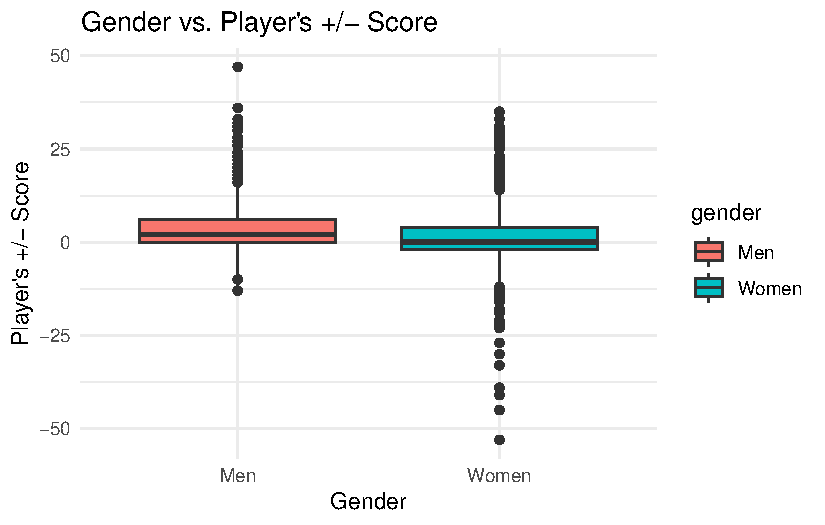
\includegraphics[keepaspectratio]{final_eda_files/figure-pdf/unnamed-chunk-4-1.pdf}}

\begin{Shaded}
\begin{Highlighting}[]
\FunctionTok{ggplot}\NormalTok{(ultimate\_data, }\FunctionTok{aes}\NormalTok{(}\AttributeTok{x =}\NormalTok{ level, }\AttributeTok{y =}\NormalTok{ plus\_minus, }\AttributeTok{fill =}\NormalTok{ level)) }\SpecialCharTok{+}
  \FunctionTok{geom\_violin}\NormalTok{(}\AttributeTok{trim =} \ConstantTok{FALSE}\NormalTok{) }\SpecialCharTok{+}
  \FunctionTok{labs}\NormalTok{(}
    \AttributeTok{title =} \StringTok{"Player\textquotesingle{}s +/{-} Score for Division 1 vs Division 3"}\NormalTok{,}
    \AttributeTok{x =} \StringTok{"Division"}\NormalTok{,}
    \AttributeTok{y =} \StringTok{"Player\textquotesingle{}s +/{-} Score"}
\NormalTok{  ) }\SpecialCharTok{+}
  \FunctionTok{scale\_fill\_manual}\NormalTok{(}\AttributeTok{values =} \FunctionTok{c}\NormalTok{(}\StringTok{"Division 1"} \OtherTok{=} \StringTok{"blue"}\NormalTok{, }\StringTok{"Division 3"} \OtherTok{=} \StringTok{"pink"}\NormalTok{)) }\SpecialCharTok{+} 
  \FunctionTok{theme\_minimal}\NormalTok{()}
\end{Highlighting}
\end{Shaded}

\pandocbounded{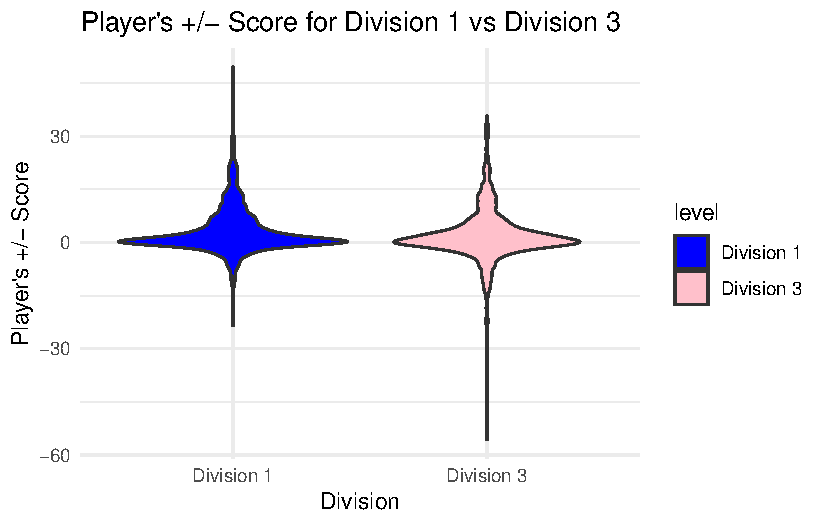
\includegraphics[keepaspectratio]{final_eda_files/figure-pdf/unnamed-chunk-5-1.pdf}}

\begin{Shaded}
\begin{Highlighting}[]
\NormalTok{ultimate\_data }\SpecialCharTok{\%\textgreater{}\%} \FunctionTok{ggplot}\NormalTok{(}\FunctionTok{aes}\NormalTok{(}\AttributeTok{x =}\NormalTok{ pts\_per\_game, }\AttributeTok{y =}\NormalTok{ plus\_minus, }\AttributeTok{color =}\NormalTok{ division)) }\SpecialCharTok{+} 
   \FunctionTok{geom\_point}\NormalTok{() }\SpecialCharTok{+} \FunctionTok{geom\_smooth}\NormalTok{(}\AttributeTok{method =} \StringTok{\textquotesingle{}lm\textquotesingle{}}\NormalTok{, }\AttributeTok{se =}\NormalTok{ F) }\SpecialCharTok{+} \FunctionTok{scale\_x\_log10}\NormalTok{() }\SpecialCharTok{+}
  \FunctionTok{labs}\NormalTok{(}\AttributeTok{x =} \StringTok{"Points per game"}\NormalTok{, }\AttributeTok{y =} \StringTok{"Plus/Minus"}\NormalTok{, }\AttributeTok{color =} \StringTok{"Division"}\NormalTok{) }\SpecialCharTok{+} 
  \FunctionTok{theme\_minimal}\NormalTok{() }\SpecialCharTok{+}
  \FunctionTok{scale\_color\_viridis\_d}\NormalTok{()}
\end{Highlighting}
\end{Shaded}

\begin{verbatim}
Warning in scale_x_log10(): log-10 transformation introduced infinite values.
log-10 transformation introduced infinite values.
\end{verbatim}

\begin{verbatim}
`geom_smooth()` using formula = 'y ~ x'
\end{verbatim}

\begin{verbatim}
Warning: Removed 550 rows containing non-finite outside the scale range
(`stat_smooth()`).
\end{verbatim}

\pandocbounded{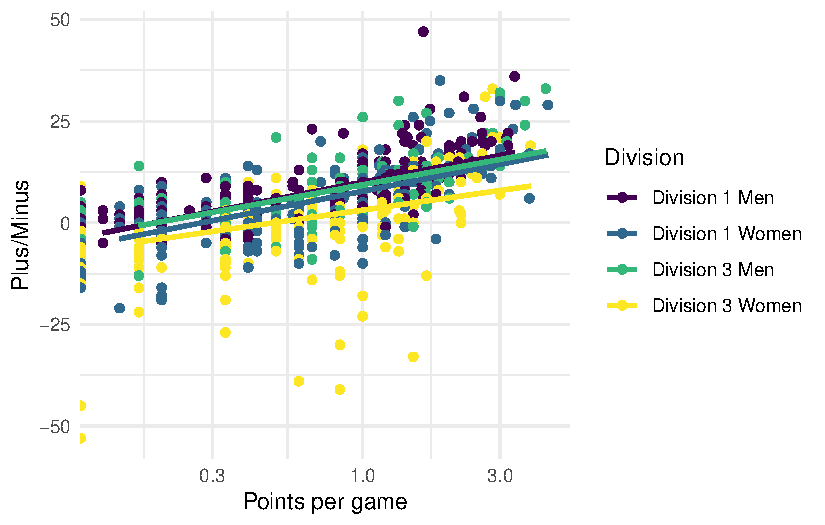
\includegraphics[keepaspectratio]{final_eda_files/figure-pdf/unnamed-chunk-6-1.pdf}}

\begin{Shaded}
\begin{Highlighting}[]
\NormalTok{ultimate\_data }\SpecialCharTok{\%\textgreater{}\%} \FunctionTok{ggplot}\NormalTok{(}\FunctionTok{aes}\NormalTok{(}\AttributeTok{x =}\NormalTok{ ds\_per\_game, }\AttributeTok{y =}\NormalTok{ plus\_minus, }\AttributeTok{color =}\NormalTok{ division)) }\SpecialCharTok{+} 
   \FunctionTok{geom\_point}\NormalTok{() }\SpecialCharTok{+} \FunctionTok{geom\_smooth}\NormalTok{(}\AttributeTok{method =} \StringTok{\textquotesingle{}lm\textquotesingle{}}\NormalTok{, }\AttributeTok{se =}\NormalTok{ F)}\SpecialCharTok{+}
  \FunctionTok{theme\_minimal}\NormalTok{() }\SpecialCharTok{+} \FunctionTok{scale\_x\_log10}\NormalTok{() }\SpecialCharTok{+} 
  \FunctionTok{labs}\NormalTok{(}\AttributeTok{x =} \StringTok{"Ds per game"}\NormalTok{, }\AttributeTok{y =} \StringTok{"Plus/Minus"}\NormalTok{, }\AttributeTok{color =} \StringTok{"Division"}\NormalTok{) }\SpecialCharTok{+}
  \FunctionTok{scale\_color\_viridis\_d}\NormalTok{()}
\end{Highlighting}
\end{Shaded}

\begin{verbatim}
Warning in scale_x_log10(): log-10 transformation introduced infinite values.
log-10 transformation introduced infinite values.
\end{verbatim}

\begin{verbatim}
`geom_smooth()` using formula = 'y ~ x'
\end{verbatim}

\begin{verbatim}
Warning: Removed 638 rows containing non-finite outside the scale range
(`stat_smooth()`).
\end{verbatim}

\pandocbounded{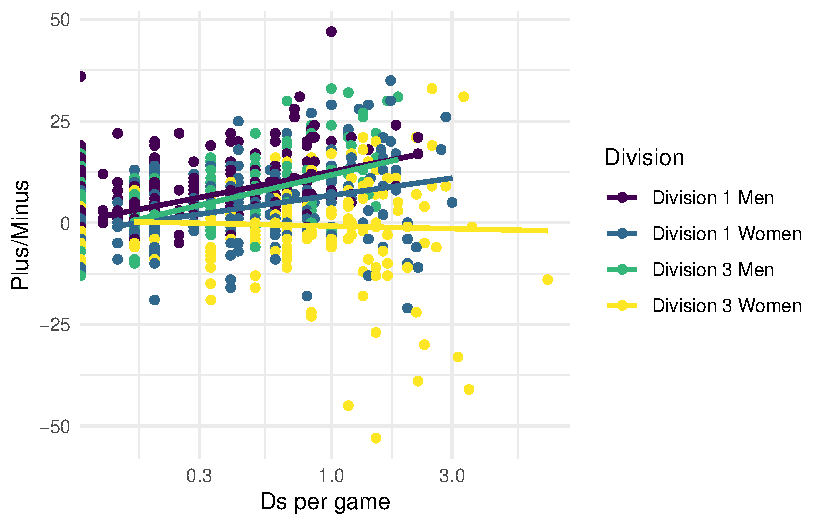
\includegraphics[keepaspectratio]{final_eda_files/figure-pdf/unnamed-chunk-6-2.pdf}}

\begin{Shaded}
\begin{Highlighting}[]
\NormalTok{ultimate\_data }\SpecialCharTok{\%\textgreater{}\%} \FunctionTok{ggplot}\NormalTok{(}\FunctionTok{aes}\NormalTok{(}\AttributeTok{x =}\NormalTok{ turns\_per\_game, }\AttributeTok{y =}\NormalTok{ plus\_minus, }\AttributeTok{color =}\NormalTok{ division)) }\SpecialCharTok{+} 
   \FunctionTok{geom\_point}\NormalTok{() }\SpecialCharTok{+} \FunctionTok{geom\_smooth}\NormalTok{(}\AttributeTok{method =} \StringTok{\textquotesingle{}lm\textquotesingle{}}\NormalTok{, }\AttributeTok{se =}\NormalTok{ F) }\SpecialCharTok{+} \FunctionTok{scale\_x\_log10}\NormalTok{() }\SpecialCharTok{+}
  \FunctionTok{labs}\NormalTok{(}\AttributeTok{x =} \StringTok{"Turns per game"}\NormalTok{, }\AttributeTok{y =} \StringTok{"Plus/Minus"}\NormalTok{, }\AttributeTok{color =} \StringTok{"Division"}\NormalTok{) }\SpecialCharTok{+} \FunctionTok{theme\_minimal}\NormalTok{() }\SpecialCharTok{+}
  \FunctionTok{scale\_color\_viridis\_d}\NormalTok{()}
\end{Highlighting}
\end{Shaded}

\begin{verbatim}
Warning in scale_x_log10(): log-10 transformation introduced infinite values.
log-10 transformation introduced infinite values.
\end{verbatim}

\begin{verbatim}
`geom_smooth()` using formula = 'y ~ x'
\end{verbatim}

\begin{verbatim}
Warning: Removed 424 rows containing non-finite outside the scale range
(`stat_smooth()`).
\end{verbatim}

\pandocbounded{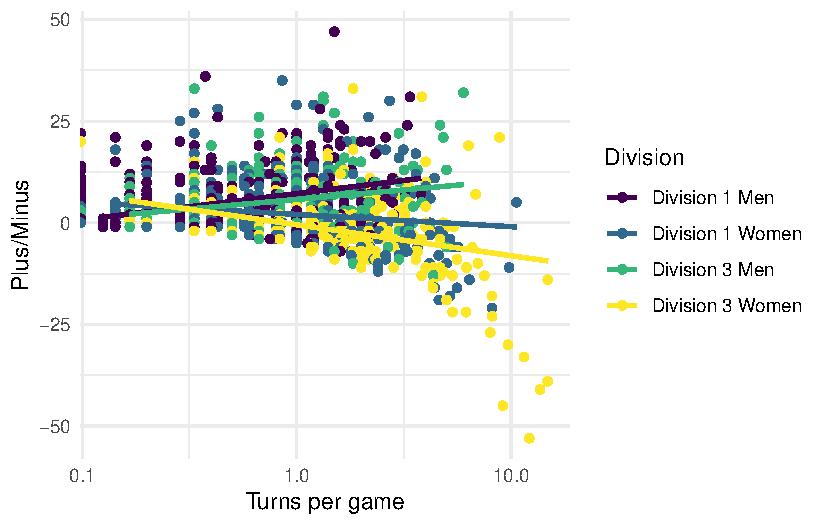
\includegraphics[keepaspectratio]{final_eda_files/figure-pdf/unnamed-chunk-6-3.pdf}}




\end{document}
